\documentclass[11pt]{article}

\usepackage[margin=0.78in]{geometry}
\usepackage[T1]{fontenc}
\usepackage[utf8]{inputenc}
\usepackage{lmodern}
\usepackage{microtype}
\usepackage{booktabs}
\usepackage{tabularx}
\usepackage{longtable}
\usepackage{array}
\usepackage{enumitem}
\usepackage{caption}
\usepackage{float}
\usepackage{xcolor}
\usepackage{seqsplit}
\usepackage{amsmath}
\usepackage{tikz}
\usepackage{pgfplots}
\usepackage{hyperref}
\usetikzlibrary{arrows.meta, positioning, calc, shapes.multipart}
\pgfplotsset{compat=1.18}

\hypersetup{
  colorlinks=true,
  linkcolor=black,
  urlcolor=blue!55!black,
  citecolor=black
}

\definecolor{BoxBlue}{RGB}{226,236,248}
\definecolor{BoxGreen}{RGB}{226,241,232}
\definecolor{BoxYellow}{RGB}{250,242,220}
\definecolor{BoxRed}{RGB}{248,226,226}
\definecolor{LineGray}{RGB}{90,90,90}
\definecolor{BarBlue}{RGB}{78,121,167}
\definecolor{BarGreen}{RGB}{89,161,79}
\definecolor{BarOrange}{RGB}{242,142,44}
\definecolor{BarRed}{RGB}{204,80,73}

\newcommand{\id}[1]{\texttt{\expandafter\seqsplit\expandafter{\detokenize{#1}}}}
\newcommand{\pct}[1]{#1\%}
\newcolumntype{Y}{>{\raggedright\arraybackslash}X}
\newcolumntype{L}[1]{>{\raggedright\arraybackslash}p{#1}}
\setlist[itemize]{leftmargin=1.3em, itemsep=0.25em}
\setlist[enumerate]{leftmargin=1.5em, itemsep=0.25em}
\captionsetup{font=small, labelfont=bf}

\title{\textbf{Commercial Name Search Benchmark V2}\\
\large Dataset, Evaluation, and Master Algorithm Briefing}
\author{medicine-search-clean}
\date{Prepared for engineering review}

\begin{document}
\maketitle

\begin{abstract}
This document explains the full V2 commercial-name search benchmark in plain
English first, then gives the engineering details needed for a team review.
V2 contains 115,000 generated test cases across 34 planned categories, evaluates
three search algorithms, and reports both retrieval quality and medical-safety
behavior. The most important idea is simple: a medical search system must not
only find possible medicines; it must also know when not to be confident.
\end{abstract}

\section{Algorithm Names}

\begin{table}[H]
\centering
\small
\begin{tabularx}{0.78\linewidth}{L{0.24\linewidth}Y}
\toprule
\textbf{Label} & \textbf{Implementation} \\
\midrule
Algorithm 1 & Current app evaluator. \\
Algorithm 2 & External English fast algorithm. \\
Algorithm 3 & Master rank-fusion algorithm. \\
\bottomrule
\end{tabularx}
\caption{Naming used throughout this document. Legacy implementation paths are
kept where they are needed for reproducibility.}
\end{table}

\section{Plain-Language Summary}

V2 is an obstacle course for medicine commercial-name search.
Instead of asking only ``does exact search work?'', it asks questions closer to
real pharmacy input:

\begin{itemize}
  \item What if the user writes a brand with a typo, missing letter, wrong vowel,
        OCR digit, keyboard slip, or phonetic spelling?
  \item What if the user writes a short prefix that can mean several different
        medicines?
  \item What if the query is a real medicine name but the route, form, or status
        makes a confident answer risky?
  \item What if the correct behavior is not ``return one answer'', but ``show
        candidates and ask for clarification''?
\end{itemize}

An analogy: V2 is like testing a navigation system in a city with wrong street
spellings, short abbreviations, duplicate street names, road closures, and
unsafe shortcuts. A normal search test checks if the system can find a street.
V2 also checks whether the system avoids sending someone down the wrong road
when two streets look almost identical.

\section{What Is In V2}

\begin{table}[H]
\centering
\small
\begin{tabularx}{\linewidth}{L{0.38\linewidth}Y}
\toprule
\textbf{File} & \textbf{Purpose} \\
\midrule
\path{benchmark_02_synthetic/generate_dataset.py} &
Deterministic generator. It encodes the 34-category plan and writes every row. \\
\path{benchmark_02_synthetic/data/test_cases.csv} &
The final 115,000-row generated dataset. \\
\path{benchmark_02_synthetic/data/category_summary.csv} &
One row per category with target count, actual count, danger split, difficulty
split, and generator function. \\
\path{benchmark_02_synthetic/evaluate_algorithms_1_2.py} &
Evaluates Algorithm 1 and Algorithm 2. \\
\path{benchmark_02_synthetic/evaluate_algorithm_3.py} &
Evaluates Algorithm 3. \\
\path{benchmark_02_synthetic/results/01_full_benchmark/algorithm_1_3_comparison.md} &
Full three-way report with every category and every detailed error-type bucket. \\
\path{benchmark_01_legacy/master_algorithms/master_commercial_name_search.py} &
Algorithm 3 implementation. \\
\bottomrule
\end{tabularx}
\caption{The practical V2 file map.}
\end{table}

\section{Dataset Totals}

The plan headline said approximately 120,000 cases, but the explicit category
targets sum to 115,000. The generator follows the explicit target rows because
they are auditable. It does not invent an undocumented 5,000-row top-up category.

\begin{table}[H]
\centering
\small
\begin{tabular}{lr}
\toprule
\textbf{Metric} & \textbf{Value} \\
\midrule
Generated rows & 115,000 \\
Planned categories & 34 \\
Detailed scope/category/error-type buckets & 4,243 \\
Hard + extreme rows & 84,400 \\
Hard + extreme ratio & 73.40\% \\
Safe rows & 80,931 \\
Caution rows & 11,144 \\
Dangerous rows & 22,925 \\
Match-behavior rows & 106,500 \\
Ambiguous-behavior rows & 5,500 \\
No-match-behavior rows & 3,000 \\
\bottomrule
\end{tabular}
\caption{Dataset size and distribution summary.}
\end{table}

\begin{figure}[H]
\centering
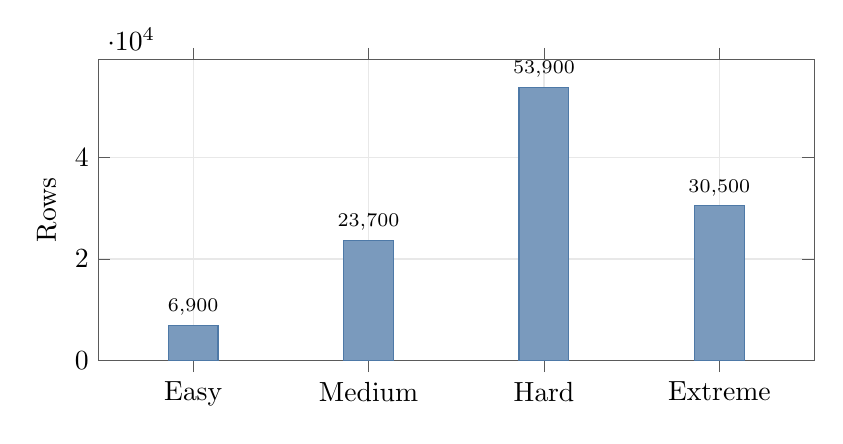
\begin{tikzpicture}
\begin{axis}[
    ybar,
    width=0.88\linewidth,
    height=5.4cm,
    ymin=0,
    ylabel={Rows},
    symbolic x coords={Easy,Medium,Hard,Extreme},
    xtick=data,
    nodes near coords,
    nodes near coords align={vertical},
    every node near coord/.append style={font=\scriptsize},
    bar width=18pt,
    enlarge x limits=0.18,
    grid=major,
    grid style={draw=gray!18},
    axis line style={draw=LineGray},
    tick style={draw=LineGray}
]
\addplot[fill=BarBlue!75, draw=BarBlue] coordinates {
    (Easy,6900)
    (Medium,23700)
    (Hard,53900)
    (Extreme,30500)
};
\end{axis}
\end{tikzpicture}
\caption{Difficulty distribution. V2 is intentionally dominated by hard and
extreme cases so exact-match success cannot hide weak typo or safety behavior.}
\end{figure}

\section{How The Dataset Is Generated}

\subsection*{Plain Explanation}

The generator starts from real catalog-derived commercial families. For each
planned category, it applies a specific deterministic transformation: for
example, replace a visually similar letter, remove one character, rewrite a
phonetic pattern, add strength text, or create a dangerous short-prefix case.

Every row is therefore traceable:

\begin{itemize}
  \item the row has a category;
  \item the row has an error type;
  \item the row has a source base group when applicable;
  \item the row names the generator function that created it;
  \item the notes field explains the mutation.
\end{itemize}

\subsection*{Generation Pipeline}

\begin{figure}[H]
\centering
\resizebox{\linewidth}{!}{%
\begin{tikzpicture}[
  node distance=1.35cm,
  box/.style={rectangle, rounded corners=2pt, draw=LineGray, align=center,
              minimum width=3.2cm, minimum height=0.9cm, font=\small},
  arrow/.style={-{Latex[length=2.4mm]}, draw=LineGray, line width=0.55pt}
]
\node[box, fill=BoxBlue] (catalog) {Catalog\\\path{canonical_candidates.csv}};
\node[box, fill=BoxBlue, right=of catalog] (index) {Build indexed\\catalog views};
\node[box, fill=BoxYellow, right=of index] (plans) {34 category\\plans};
\node[box, fill=BoxYellow, right=of plans] (gens) {Run named\\generators};
\node[box, fill=BoxGreen, below=of gens] (select) {Deduplicate and\\stable-hash sample};
\node[box, fill=BoxGreen, left=of select] (difficulty) {Assign exact\\difficulty quotas};
\node[box, fill=BoxRed, left=of difficulty] (validate) {Validate counts,\\coverage, safety ratio};
\node[box, fill=BoxBlue, left=of validate] (outputs) {Write CSV, summary,\\JSON audit};

\draw[arrow] (catalog) -- (index);
\draw[arrow] (index) -- (plans);
\draw[arrow] (plans) -- (gens);
\draw[arrow] (gens) -- (select);
\draw[arrow] (select) -- (difficulty);
\draw[arrow] (difficulty) -- (validate);
\draw[arrow] (validate) -- (outputs);
\end{tikzpicture}%
}
\caption{Actual generation flow implemented by
\protect\path{generate_dataset.py}.}
\end{figure}

\subsection*{Why Deterministic Code Instead Of Random Cases}

Random mutation would create unstable test results. That is unacceptable for a
medical search benchmark because a failure must be reproducible and explainable.
V2 uses deterministic rules and stable SHA-256 sampling. The sampling still
avoids catalog-order bias, but repeated runs produce the same dataset.

\section{Dataset Row Schema}

The CSV keeps legacy evaluation columns first, then adds provenance columns.
The most important fields are:

\begin{table}[H]
\centering
\small
\begin{tabularx}{\linewidth}{L{0.22\linewidth}L{0.25\linewidth}Y}
\toprule
\textbf{Column} & \textbf{Example} & \textbf{Meaning} \\
\midrule
\id{input} & \id{sharcodoll} & The simulated user query. \\
\id{expected} & \id{CHARCODOLL} & Expected commercial family, or a sentinel such as \id{__AMBIGUOUS__}. \\
\id{category} & \id{multi_char_phonetic_confusion} & High-level test case family. \\
\id{error_type} & \id{multi_phonetic_ch_to_sh_pos_0} & Detailed mutation bucket. \\
\id{difficulty} & \id{EXTREME} & Difficulty label assigned from category quotas. \\
\id{danger} & \id{SAFE}, \id{CAUTION}, or \id{DANGEROUS} & Medical risk label. \\
\id{expected_behavior} & \id{match}, \id{ambiguous}, or \id{no_match} & What behavior the evaluator expects. \\
\id{generator_function} & \id{generate_multi_char_phonetic_confusion} & Exact function that generated the row. \\
\id{collision_with} & \id{ABC LEMON HONEY; ABC OMEGA} & Other families that collide with the query, when relevant. \\
\id{notes} & Mutation explanation & Human-readable provenance. \\
\bottomrule
\end{tabularx}
\caption{Core V2 dataset columns.}
\end{table}

\section{All V2 Categories}

\scriptsize
\setlength{\tabcolsep}{2.4pt}
\begin{longtable}{rL{0.10\linewidth}L{0.22\linewidth}rL{0.20\linewidth}L{0.24\linewidth}}
\caption{All 34 planned V2 categories. Every row is generated by the listed function.}\\
\toprule
\textbf{\#} & \textbf{Scope} & \textbf{Category} & \textbf{Rows} & \textbf{Generator} & \textbf{Purpose} \\
\midrule
\endfirsthead
\toprule
\textbf{\#} & \textbf{Scope} & \textbf{Category} & \textbf{Rows} & \textbf{Generator} & \textbf{Purpose} \\
\midrule
\endhead
1 & inside & \id{single_letter_visual_confusion} & 8,000 & \id{generate_single_letter_visual_confusion} & Replace one letter with a visually similar one. \\
2 & inside & \id{single_letter_phonetic_confusion} & 6,000 & \id{generate_single_letter_phonetic_confusion} & Replace one letter with an Egyptian-Arabic sound-alike. \\
3 & inside & \id{multi_char_phonetic_confusion} & 5,000 & \id{generate_multi_char_phonetic_confusion} & Rewrite multi-character patterns such as \id{ch} to \id{sh}. \\
4 & inside & \id{ligature_confusion} & 4,000 & \id{generate_ligature_confusion} & Merge or split visually similar adjacent letters. \\
5 & inside & \id{single_char_deletion_position_weighted} & 5,000 & \id{generate_single_char_deletion_position_weighted} & Delete one character with planned position weights. \\
6 & inside & \id{single_char_insertion} & 3,000 & \id{generate_single_char_insertion} & Insert an extra character, duplicate, or adjacent-key letter. \\
7 & inside & \id{transposition_position_weighted} & 3,000 & \id{generate_transposition_position_weighted} & Swap adjacent letters with weighted positions. \\
8 & inside & \id{truncation_doctor_abbreviation} & 6,000 & \id{generate_truncation_doctor_abbreviation} & Use only the first 3--6 compact characters. \\
9 & inside & \id{two_error_combinations} & 8,000 & \id{generate_two_error_combinations} & Chain two realistic corruptions. \\
10 & inside & \id{three_error_combinations} & 5,000 & \id{generate_three_error_combinations} & Chain three realistic corruptions. \\
11 & inside & \id{speed_typing_errors} & 3,000 & \id{generate_speed_typing_errors} & Simulate repeated or skipped letters from fast typing. \\
12 & inside & \id{wrong_vowels_in_consonant_frame} & 5,000 & \id{generate_wrong_vowels_in_consonant_frame} & Keep consonants but guess vowels incorrectly. \\
13 & inside & \id{punctuation_whitespace_copy_paste_artifacts} & 1,000 & \id{generate_punctuation_whitespace_copy_paste_artifacts} & Add copy-paste punctuation and spacing noise. \\
14 & inside & \id{case_sensitivity} & 500 & \id{generate_case_sensitivity} & Vary upper/lower/title/mixed case. \\
15 & inside & \id{number_word_confusion} & 500 & \id{generate_number_word_confusion} & Rewrite digits as words or spaced forms. \\
16 & semi\_outside & \id{embedded_form_strength_parsing} & 4,000 & \id{generate_embedded_form_strength_parsing} & Mix brand text with form and strength tokens. \\
17 & safety & \id{dangerous_ed1_pairs} & 5,000 & \id{generate_dangerous_ed1_pairs} & One-edit-apart catalog pairs with different ingredients. \\
18 & safety & \id{substring_traps} & 3,000 & \id{generate_substring_traps} & Short real drug is prefix of longer different drug. \\
19 & safety & \id{negative_no_match_expected} & 3,000 & \id{generate_negative_no_match_expected} & Inputs that should not become confident medicine matches. \\
20 & safety & \id{contradictory_form_route} & 2,000 & \id{generate_contradictory_form_route} & Real brand with conflicting form or route context. \\
21 & safety & \id{cancelled_na_drug_lookup} & 1,000 & \id{generate_cancelled_na_drug_lookup} & Cancelled, illegal import, N/A, or warning-status products. \\
22 & safety & \id{score_gap_ambiguity_detection} & 4,000 & \id{generate_score_gap_ambiguity_detection} & Proxy for close score-gap ambiguity using catalog collisions. \\
23 & inside & \id{ocr_letter_digit_confusion} & 4,000 & \id{generate_ocr_letter_digit_confusion} & OCR substitutions such as O/0, B/8, I/1. \\
24 & inside & \id{ocr_plus_other_error_combined} & 3,000 & \id{generate_ocr_plus_other_error_combined} & OCR error followed by another typo. \\
25 & inside & \id{double_letter_reduction_expansion} & 3,000 & \id{generate_double_letter_reduction_expansion} & Reduce double letters or double single letters. \\
26 & inside & \id{keyboard_adjacent_sampled} & 2,000 & \id{generate_keyboard_adjacent_sampled} & Sample QWERTY adjacent-key substitutions. \\
27 & inside & \id{four_plus_error_combinations} & 4,000 & \id{generate_four_plus_error_combinations} & Four or more simultaneous corruptions. \\
28 & inside & \id{consonant_frame_wrong_vowels_heavy} & 4,000 & \id{generate_consonant_frame_wrong_vowels_heavy} & Nearly all vowels wrong, consonant clues remain. \\
29 & inside & \id{multi_word_name_fragmentation} & 2,000 & \id{generate_multi_word_name_fragmentation} & Merge, abbreviate, or drop parts of multi-word names. \\
30 & inside & \id{autocorrect_artifacts} & 2,000 & \id{generate_autocorrect_artifacts} & Phone-style autocorrect and word-boundary artifacts. \\
31 & smoke & \id{exact_match_baseline} & 2,000 & \id{generate_exact_match_baseline} & Exact commercial names as a regression baseline. \\
32 & smoke & \id{exact_match_with_strength} & 2,000 & \id{generate_exact_match_with_strength} & Exact commercial names with real strength tokens. \\
33 & smoke & \id{keyboard_shift_whole_word} & 500 & \id{generate_keyboard_shift_whole_word} & Whole compact name typed one keyboard key left or right. \\
34 & smoke & \id{prefix_ambiguity_awareness} & 1,500 & \id{generate_prefix_ambiguity_awareness} & Very short prefixes should be treated as ambiguous. \\
\bottomrule
\end{longtable}
\normalsize
\setlength{\tabcolsep}{6pt}

\section{Difficulty And Danger Labels}

\subsection*{Difficulty}

Difficulty is assigned from the category plan after sampling, not guessed by
the evaluator. This matters because each category has an intended distribution.
For example, exact-match baseline is intentionally easy, while four-plus-error
combinations are mostly extreme.

The difficulty labels mean:

\begin{itemize}
  \item \textbf{Easy}: exact or near-exact input, mainly a regression guard.
  \item \textbf{Medium}: one simple issue, such as a mild typo or context token.
  \item \textbf{Hard}: realistic query corruption that needs robust retrieval.
  \item \textbf{Extreme}: several corruptions, dangerous ambiguity, or barely
        readable input.
\end{itemize}

\subsection*{Danger}

Danger is about patient-safety risk, not string edit distance alone.

\begin{itemize}
  \item \textbf{Safe}: ordinary typo or formatting issue; a wrong match is less
        likely to point confidently to a different medicine.
  \item \textbf{Caution}: ambiguity, short prefix, form/route context, or
        fragmentation where clarification is safer than certainty.
  \item \textbf{Dangerous}: a confident wrong top-1 could point to a different
        ingredient, a substring trap, or a query that should not match any drug.
\end{itemize}

The generator starts with each category's default danger. Then generated
collisions can upgrade a row. For example, the input \id{abc} for
\id{ABC IMMUNE} collides with \id{ABC LEMON HONEY}, \id{ABC MOCOTIVE}, and
\id{ABC OMEGA}; that is why it is marked dangerous even though it is only three
letters.

\section{Concrete Worked Example}

\subsection*{The Example}

Use one real V2 row:

\begin{table}[H]
\centering
\small
\begin{tabularx}{\linewidth}{L{0.28\linewidth}Y}
\toprule
\textbf{Field} & \textbf{Value} \\
\midrule
Input & \id{sharcodoll} \\
Expected & \id{CHARCODOLL} \\
Category & \id{multi_char_phonetic_confusion} \\
Error type & \id{multi_phonetic_ch_to_sh_pos_0} \\
Difficulty & \id{EXTREME} \\
Danger & \id{SAFE} \\
Expected behavior & \id{match} \\
Generator & \id{generate_multi_char_phonetic_confusion} \\
Note & The source starts with \id{CH}; the generator rewrites that sound as \id{SH}. \\
\bottomrule
\end{tabularx}
\caption{One row from \protect\path{data/test_cases.csv}.}
\end{table}

\subsection*{How This Row Is Created}

\begin{figure}[H]
\centering
\resizebox{0.95\linewidth}{!}{%
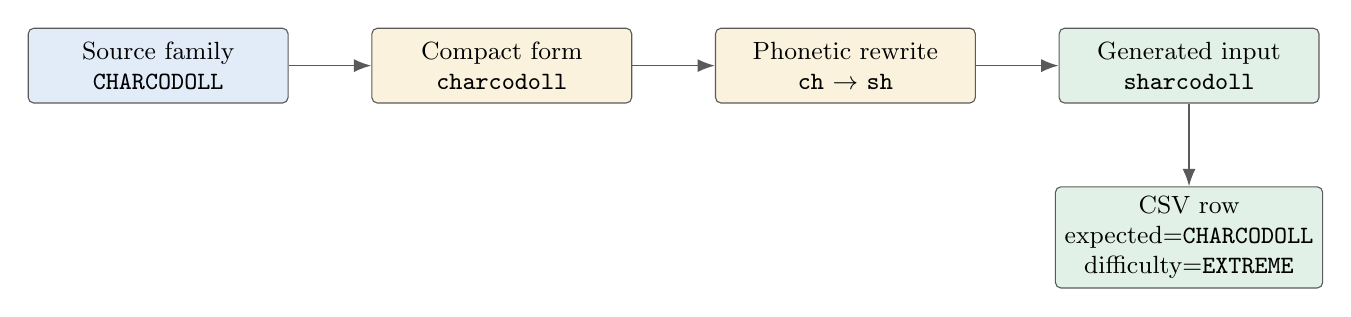
\begin{tikzpicture}[
  node distance=1.05cm,
  box/.style={rectangle, rounded corners=2pt, draw=LineGray, align=center,
              minimum width=3.3cm, minimum height=0.95cm, font=\small},
  arrow/.style={-{Latex[length=2.2mm]}, draw=LineGray, line width=0.55pt}
]
\node[box, fill=BoxBlue] (source) {Source family\\\id{CHARCODOLL}};
\node[box, fill=BoxYellow, right=of source] (compact) {Compact form\\\id{charcodoll}};
\node[box, fill=BoxYellow, right=of compact] (mutation) {Phonetic rewrite\\\id{ch} $\rightarrow$ \id{sh}};
\node[box, fill=BoxGreen, right=of mutation] (output) {Generated input\\\id{sharcodoll}};
\node[box, fill=BoxGreen, below=of output] (csv) {CSV row\\expected=\id{CHARCODOLL}\\difficulty=\id{EXTREME}};

\draw[arrow] (source) -- (compact);
\draw[arrow] (compact) -- (mutation);
\draw[arrow] (mutation) -- (output);
\draw[arrow] (output) -- (csv);
\end{tikzpicture}%
}
\caption{The worked example from catalog name to generated test case.}
\end{figure}

\subsection*{How The Algorithms Behaved}

\begin{table}[H]
\centering
\small
\begin{tabularx}{\linewidth}{L{0.21\linewidth}rrrrL{0.19\linewidth}Y}
\toprule
\textbf{Algorithm} & \textbf{Rank} & \textbf{Hit@1} & \textbf{Hit@20} &
\textbf{Unsafe} & \textbf{Top 1} & \textbf{Status / note} \\
\midrule
Algorithm 1 & 1 & 1 & 1 & 0 & \id{CHARCODOLL} &
Finds the right family but returns a clarification-style result. \\
Algorithm 2 & 1 & 1 & 1 & 0 & \id{CHARCODOLL} &
Finds the right family with low confidence. \\
Algorithm 3 & 1 & 1 & 1 & 0 & \id{CHARCODOLL} &
Merges both signals, keeps retrieval success, and stays ambiguous because
the safety gate does not force confidence. \\
\bottomrule
\end{tabularx}
\caption{Row-level result for \texttt{sharcodoll}.}
\end{table}

Plain interpretation: both child algorithms recover the intended family.
The master keeps that recovery, but it does not pretend the answer is safe
enough for automatic confident top-1 dispensing. That is acceptable for a
\id{match} row because behavior success requires the relevant family in the
candidate list, not forced confidence.

\section{Representative Test Cases}

\begin{table}[H]
\centering
\small
\begin{tabularx}{\linewidth}{L{0.23\linewidth}L{0.25\linewidth}L{0.18\linewidth}Y}
\toprule
\textbf{Input} & \textbf{Expected output} & \textbf{Category} & \textbf{What it exercises} \\
\midrule
\id{sharcodoll} & \id{CHARCODOLL} & \id{multi_char_phonetic_confusion} &
Sound-alike rewrite: \id{CH} becomes \id{SH}. \\
\id{abc} & \id{ABC IMMUNE} & \id{truncation_doctor_abbreviation} &
Short doctor-style prefix with several colliding families. \\
\id{abimol} & \id{ABIMOL EXTRA} & \id{substring_traps} &
Dangerous case where a short real drug is also a prefix of a longer family. \\
\id{112} & \id{__NO_MATCH__} & \id{negative_no_match_expected} &
Metadata-like input should not produce a confident medicine match. \\
\id{aape renewal sunscreen spf 60ml} & \id{AAPE RENEWAL SUNSCREEN SPF} &
\id{embedded_form_strength_parsing} & Brand plus strength/form context. \\
\bottomrule
\end{tabularx}
\caption{Representative V2 examples.}
\end{table}

\section{Evaluation Semantics}

V2 separates \textbf{retrieval success} from \textbf{safety behavior}.

\begin{itemize}
  \item Retrieval asks: did the expected or relevant family appear at rank 1,
        5, 10, or 20?
  \item Behavior asks: did the algorithm respond in the right mode: confident
        match, clarification/ambiguous, or no confident match?
\end{itemize}

This distinction is important. In a dangerous prefix case, returning the right
family somewhere in the list is useful. Returning one confident wrong family at
rank 1 is unsafe.

\begin{table}[H]
\centering
\small
\begin{tabularx}{\linewidth}{L{0.19\linewidth}Y}
\toprule
\textbf{Metric} & \textbf{Meaning} \\
\midrule
Hit@1 / Hit@20 & Whether a relevant target appears at rank 1 or within the top 20. \\
MRR@20 & Reciprocal rank of the first relevant target inside the top 20. \\
Behavior success & Whether the algorithm matched the row's intended behavior: match, ambiguous, or no-match. \\
Unsafe confident top-1 & A confident top-1 result exists, but it is not relevant and is not marked for clarification. \\
Missing clarification & A caution/danger row should avoid confidence, but the algorithm does not. \\
\bottomrule
\end{tabularx}
\caption{The main evaluation metrics.}
\end{table}

\section{Headline Results}

\begin{table}[H]
\centering
\small
\begin{tabular}{lrrrr}
\toprule
\textbf{Scope} & \textbf{Cases} & \textbf{Algorithm 1 Hit@20} & \textbf{Algorithm 2 Hit@20} & \textbf{Algorithm 3 Hit@20} \\
\midrule
inside & 87,000 & 87.02\% & 92.00\% & 92.41\% \\
safety & 18,000 & 89.86\% & 92.50\% & 93.67\% \\
semi\_outside & 4,000 & 96.97\% & 87.70\% & 97.32\% \\
smoke & 6,000 & 98.38\% & 90.25\% & 98.47\% \\
all & 115,000 & 88.40\% & 91.84\% & 93.09\% \\
\bottomrule
\end{tabular}
\caption{Top-20 retrieval by scope.}
\end{table}

\begin{figure}[H]
\centering
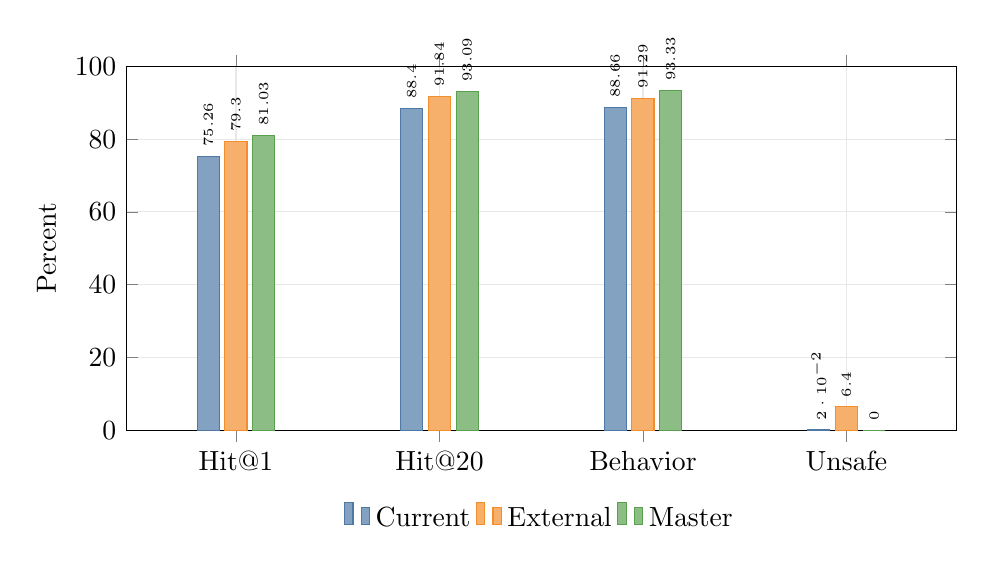
\begin{tikzpicture}
\begin{axis}[
    ybar,
    width=\linewidth,
    height=6.2cm,
    ymin=0,
    ymax=100,
    ylabel={Percent},
    symbolic x coords={Hit@1,Hit@20,Behavior,Unsafe},
    xtick=data,
    bar width=8pt,
    enlarge x limits=0.18,
    legend style={at={(0.5,-0.18)}, anchor=north, legend columns=3, draw=none},
    nodes near coords,
    every node near coord/.append style={font=\tiny, rotate=90, anchor=west},
    grid=major,
    grid style={draw=gray!18}
]
\addplot[fill=BarBlue!70, draw=BarBlue] coordinates {
    (Hit@1,75.26) (Hit@20,88.40) (Behavior,88.66) (Unsafe,0.02)
};
\addplot[fill=BarOrange!70, draw=BarOrange] coordinates {
    (Hit@1,79.30) (Hit@20,91.84) (Behavior,91.29) (Unsafe,6.40)
};
\addplot[fill=BarGreen!70, draw=BarGreen] coordinates {
    (Hit@1,81.03) (Hit@20,93.09) (Behavior,93.33) (Unsafe,0.00)
};
\legend{Current,External,Master}
\end{axis}
\end{tikzpicture}
\caption{Overall V2 comparison. Unsafe is also a percentage; lower is better.}
\end{figure}

\section{Algorithm 3}

\subsection*{Plain Explanation}

Algorithm 3 is a reviewer that listens to two specialists:

\begin{itemize}
  \item Algorithm 1, which is safer around clarification, prefix risk,
        form/route context, and strength-heavy queries;
  \item Algorithm 2, which is stronger on many typo-heavy
        commercial-name retrieval cases.
\end{itemize}

Algorithm 3 does not blindly choose one. It merges their ranked candidates by
commercial family, scores the merged candidates, then applies safety gates before
deciding whether the response is confident or ambiguous.

\subsection*{Fusion Flow}

\begin{figure}[H]
\centering
\resizebox{\linewidth}{!}{%
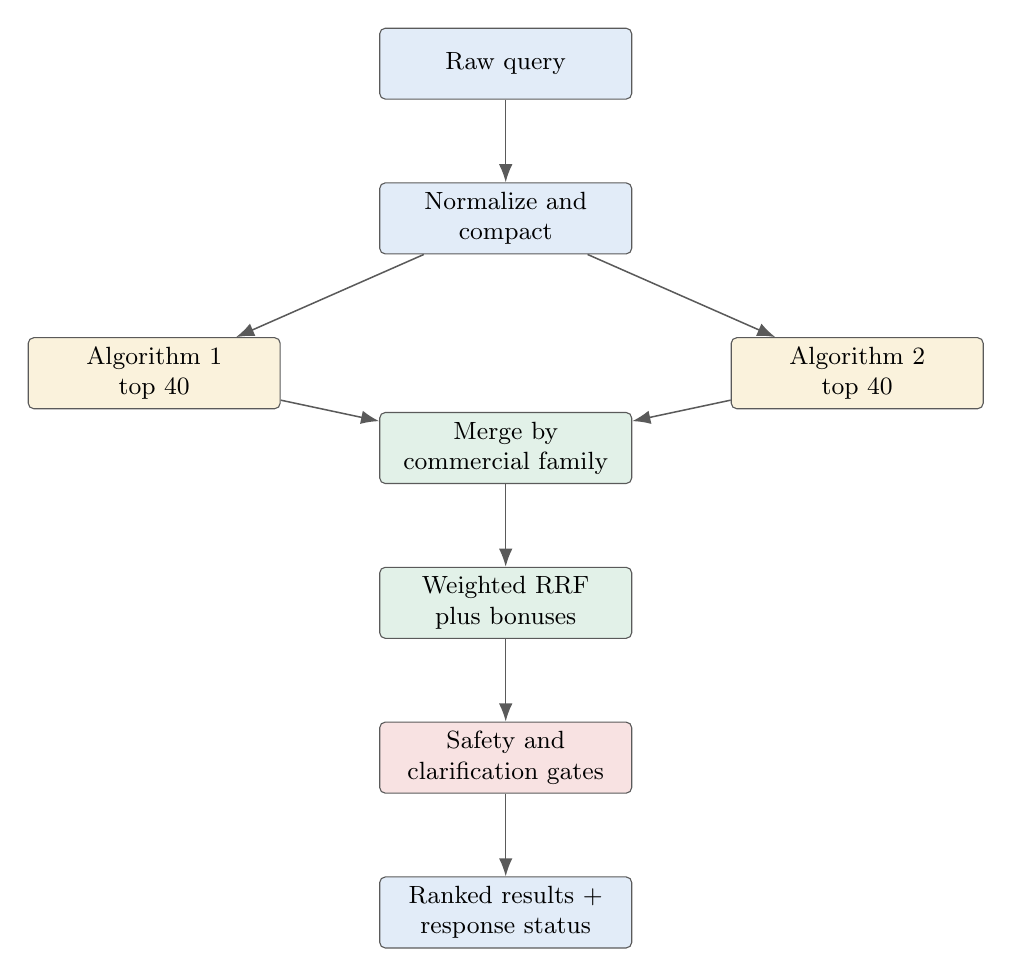
\begin{tikzpicture}[
  node distance=1.05cm and 1.25cm,
  box/.style={rectangle, rounded corners=2pt, draw=LineGray, align=center,
              minimum width=3.2cm, minimum height=0.9cm, font=\small},
  arrow/.style={-{Latex[length=2.3mm]}, draw=LineGray, line width=0.55pt}
]
\node[box, fill=BoxBlue] (query) {Raw query};
\node[box, fill=BoxBlue, below=of query] (normalize) {Normalize and\\compact};
\node[box, fill=BoxYellow, below left=of normalize] (current) {Algorithm 1\\top 40};
\node[box, fill=BoxYellow, below right=of normalize] (external) {Algorithm 2\\top 40};
\node[box, fill=BoxGreen, below=2.0cm of normalize] (merge) {Merge by\\commercial family};
\node[box, fill=BoxGreen, below=of merge] (score) {Weighted RRF\\plus bonuses};
\node[box, fill=BoxRed, below=of score] (safety) {Safety and\\clarification gates};
\node[box, fill=BoxBlue, below=of safety] (response) {Ranked results +\\response status};

\draw[arrow] (query) -- (normalize);
\draw[arrow] (normalize) -- (current);
\draw[arrow] (normalize) -- (external);
\draw[arrow] (current) -- (merge);
\draw[arrow] (external) -- (merge);
\draw[arrow] (merge) -- (score);
\draw[arrow] (score) -- (safety);
\draw[arrow] (safety) -- (response);
\end{tikzpicture}%
}
\caption{Master algorithm flow. The safety gate comes after retrieval, so the
master can recover candidates without automatically becoming confident.}
\end{figure}

\subsection*{Scoring}

For each merged family candidate, the master computes a weighted reciprocal-rank
fusion score:

\[
\text{score} =
\frac{w_\text{current}}{K + r_\text{current}} +
\frac{w_\text{external}}{K + r_\text{external}} +
\text{small child-score additions} +
\text{agreement/exact/context bonuses}.
\]

In the implementation, \(K = 8.0\). The rank weights depend on query shape:

\begin{table}[H]
\centering
\small
\begin{tabularx}{\linewidth}{L{0.33\linewidth}rrY}
\toprule
\textbf{Query shape} & \textbf{Algorithm 1 weight} & \textbf{Algorithm 2 weight} & \textbf{Reason} \\
\midrule
Short compact query, length \(\leq 4\), no numbers & 1.60 & 0.55 &
Short prefixes collide with many unrelated families, so conservative behavior matters more. \\
Context-heavy query with numbers, routes, or many tokens & 1.45 & 0.78 &
Algorithm 1 handles strength/form/route context better. \\
Ordinary brand-like typo & 1.00 & 1.22 &
Algorithm 2 is stronger on typo retrieval. \\
\bottomrule
\end{tabularx}
\caption{The main rank-weight regimes.}
\end{table}

\subsection*{Safety Gates}

Algorithm 3 separates ``candidate is useful'' from ``candidate is safe to answer
confidently.'' A candidate can be ranked high and still require clarification.

Algorithm 3 marks a candidate as requiring clarification when:

\begin{itemize}
  \item Algorithm 1 already asked for clarification;
  \item the compact query is extremely short;
  \item the candidate appears only in Algorithm 2 results;
  \item the candidate lacks exact Algorithm 1 evidence or high-rank agreement.
\end{itemize}

It allows confidence only when there is strong support, such as exact Algorithm 1
evidence at rank 1 or both algorithms agreeing in the top 3 without an Algorithm 1
clarification flag.

\section{Why Algorithm 3 Improved V2}

Algorithm 2 had stronger typo retrieval but a high unsafe confident top-1 rate:
6.40\% overall and 13.42\% in the safety scope. Algorithm 1 was much safer but
weaker on many heavy typo categories. Algorithm 3 combines Algorithm 2's
retrieval advantage with Algorithm 1's safety behavior.

\begin{table}[H]
\centering
\small
\begin{tabular}{lrrr}
\toprule
\textbf{Overall metric} & \textbf{Algorithm 1} & \textbf{Algorithm 2} & \textbf{Algorithm 3} \\
\midrule
Hit@1 & 75.26\% & 79.30\% & 81.03\% \\
Hit@20 & 88.40\% & 91.84\% & 93.09\% \\
Behavior success & 88.66\% & 91.29\% & 93.33\% \\
Unsafe confident top-1 & 0.02\% & 6.40\% & 0.00\% \\
Average candidate pool & 188.85 & 17.86 & 37.69 \\
\bottomrule
\end{tabular}
\caption{Overall V2 result across 115,000 cases.}
\end{table}

Algorithm 3 is not expected to beat the best child in every category. In some
clean typo buckets, Algorithm 2 still has the best raw Hit@1. Algorithm 3's
value is the combined system behavior: stronger overall retrieval,
better behavior success, and zero unsafe confident top-1 on V2.

\section{Coverage Contract}

The V2 reports are designed not to skip categories.

\begin{table}[H]
\centering
\small
\begin{tabular}{lr}
\toprule
\textbf{Audit check} & \textbf{Result} \\
\midrule
Dataset rows & 115,000 \\
Current-app result rows & 115,000 \\
External result rows & 115,000 \\
Master result rows & 115,000 \\
Dataset categories & 34 \\
Metric category buckets & 34 \\
Missing category buckets & 0 \\
Dataset detailed error-type buckets & 4,243 \\
Metric detailed error-type buckets & 4,243 \\
Missing error-type buckets & 0 \\
Blank category context cells & 0 \\
Blank error-type context cells & 0 \\
\bottomrule
\end{tabular}
\caption{No-skipping audit summary.}
\end{table}

\section{Reproduction Commands}

Run these from \path{medicine-search-clean}:

\begin{verbatim}
PYTHONDONTWRITEBYTECODE=1 \
python3 'benchmark_02_synthetic/generate_dataset.py'

PYTHONDONTWRITEBYTECODE=1 \
python3 'benchmark_02_synthetic/evaluate_algorithms_1_2.py' \
  --workers 8 --chunk-size 200

PYTHONDONTWRITEBYTECODE=1 \
python3 'benchmark_02_synthetic/evaluate_algorithm_3.py' \
  --workers 8 --chunk-size 200
\end{verbatim}

The committed full Algorithm 3 run evaluated 115,000 rows with 8 workers and chunk
size 200 in 161.88 seconds.

\section{Engineering Takeaways}

\begin{itemize}
  \item V2 is generated by code, not hand-curated rows.
  \item Every category has a named generator function and exact output count.
  \item The dataset is intentionally hard: 73.40\% of rows are hard or extreme.
  \item Safety is measured separately from retrieval because medical search can
        be wrong even when it retrieves plausible candidates.
  \item Algorithm 3 improves overall Hit@1, Hit@20, and
        behavior success while eliminating unsafe confident top-1 on V2.
  \item The full Markdown and CSV reports include every category and all 4,243
        detailed error-type buckets.
\end{itemize}

\end{document}
